% Airborne magnetic analysis: Basement depths and sediment thickness

\section*{Abstract}

New geophysical data from Antarctica's Ross Embayment reveal the structure and subglacial geology of extended continental crust beneath the Ross Ice Shelf. We use airborne magnetic data from the ROSETTA-Ice Project to locate the contact between magnetic basement and overlying sediments. We delineate a broad, segmented basement high with thin (0-500~m) non-magnetic sedimentary cover which trends northward into the Ross Sea's Central High. Before subsiding in the Oligocene, this feature likely facilitated early glaciation in the region and subsequently acted as a pinning point and ice flow divide. Flanking the high are wide sedimentary basins, up to 3700~m deep, which parallel the Ross Sea basins and likely formed during Cretaceous-Neogene intracontinental extension. NW-SE basins beneath the Siple Coast grounding zone, by contrast, are narrow, deep, and elongate. They suggest tectonic divergence upon active faults that may localize geothermal heat and/or groundwater flow, both important components of the subglacial system.

\section*{Plain Language Summary}

The bedrock geology of Antarctica’s southern Ross Embayment is concealed by 100s-1000s of meters of sedimentary deposits, seawater, and the floating Ross Ice Shelf (RIS). Our research strips away those layers to discover the shape of the consolidated bedrock below, which we refer to as the basement. To do this, we use the contrast between non-magnetic sediments and magnetic basement rocks to map out the depth of the basement surface under the RIS. Our primary data source is airborne measurements of the variation in Earth’s magnetic field across the ice shelf, from flight lines spaced 10~km apart. We use the resulting basement topography to highlight sites of possible influence upon the Antarctic Ice Sheet and to further understand the tectonic history of the region. We discover contrasting basement characteristics on either side of the ice shelf, separated by an N-S trending basement high. The West Antarctic side displays evidence of active faults, which may localize geothermal heat, accommodate movements of the solid earth caused by changes in the size of the Antarctic Ice Sheet, and control the flow of groundwater between the ice base and aquifers. This work addresses critical interactions between ice and the solid earth.

\paragraph*{Key Points:}

\begin{enumerate}
    \item Aeromagnetic analysis reveals basement surface and evidence of fault-controlled extensional basins beneath Antarctica's Ross Ice Shelf (RIS).
    \item Active faults at Siple Coast likely influence ice streams through control of geothermal heat, groundwater, and glacioisostatic adjustments.
    \item A basement high beneath RIS spatially coincides with a lithospheric boundary, with contrasting sedimentary basins on either side.
\end{enumerate}


\section{Introduction} \label{chp2:intro}

The southern sector of Antarctica's Ross Embayment beneath the Ross Ice Shelf (RIS; area $\sim$480,000~km\textsuperscript{2}) is poorly resolved because the region is not accessible to conventional seismic or geophysical surveying. Rock exposures on land suggest that Ross Ice Shelf (RIS) crust consists of early Paleozoic post-orogenic sediments, intruded in places by mid-Paleozoic and Cretaceous granitoids \citep{luyendykeastern2003, goodgegeological2020}. Following the onset of extension in the mid-Cretaceous, grabens formed and filled with terrestrial and marine deposits, continuing into the Cenozoic \citep[e.g.][]{sorlienoligocene2007, coenenpaleogene2019}, as the Ross Embayment underwent thermal subsidence \citep{karnergravity2005, wilsonwest2009}. The physiography of this region then responded to the onset of glaciation in the Oligocene \citep{paxmanreconstructions2019}, coinciding with localized extension in the western Ross Sea until 11~Ma \citep{granotlate2018}. The Oligocene-early-Miocene paleo-landscape of the Ross Sea sector was revealed by marine seismic data \citep[e.g.][]{brancolinidescriptive1995, pérezearly2021} and offshore drilling that penetrated crystalline basement \citep[DSDP Site 270;][]{fordbasement1975} (Figure \ref{fig:chp2_Bathy_Mag}). Recognition of the role of elevated topography in Oligocene formation of the Antarctic Ice Sheet \citep{decontocoupled2003, wilsoninitiation2013} and the likely influence of subglacial topography upon ice sheet processes during some climate states \citep{austermannimpact2015, colleonicontinental2018} motivated our effort to determine basement topography beneath the Ross Ice Shelf.\\

\begin{figure}
    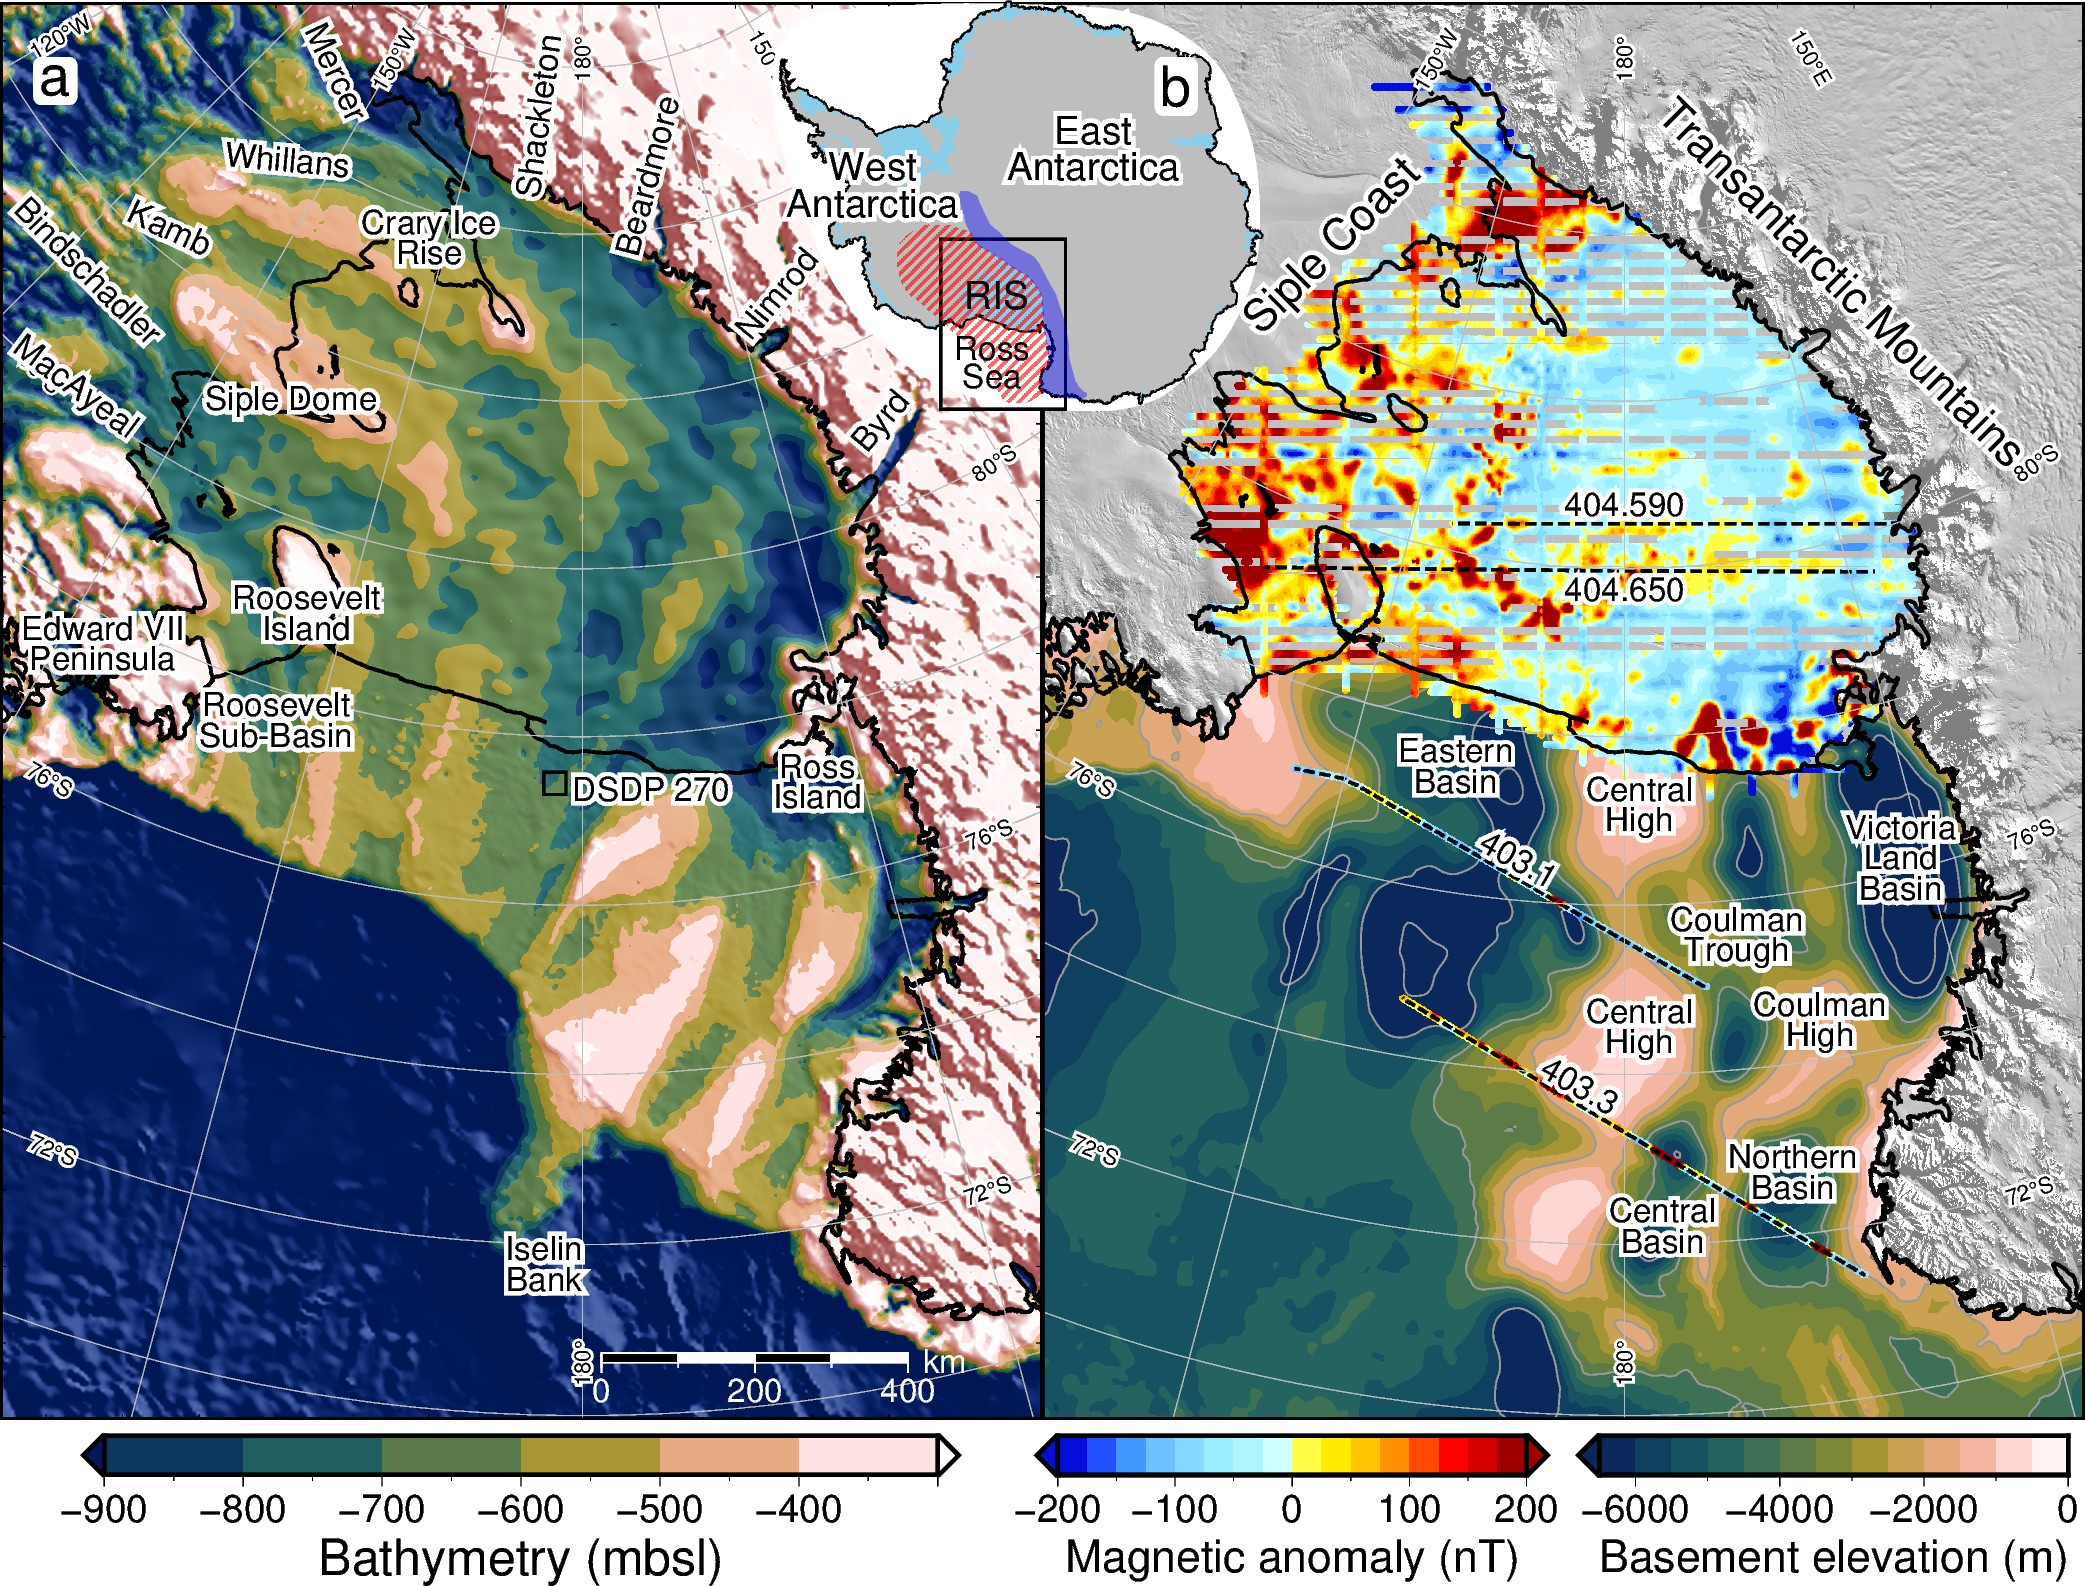
\includegraphics[width=\textwidth]{figures/chp2/Fig1_Bathy_Mag.jpg}
    \caption[Bathymetry, magnetics, and acoustic basement]{\textbf{(a)} Bathymetry and sub-ice bed elevations \citep{morlighemdeep2020} including ROSETTA-Ice gravity-derived bathymetry \citep{tintoross2019} beneath the Ross Ice Shelf (RIS). Labels include ice streams and outlet glaciers. \textbf{(b)} Basement elevation from Antarctic Offshore Stratigraphy project marine seismic compilation in the Ross Sea \citet{brancolinidescriptive1995} and airborne magnetic data from ROSETTA-Ice (over RIS) and Operation IceBridge (black dashed lines). Inset map shows figure location, West Antarctic Rift System (hatched red), Transantarctic Mountains (dark blue), and ice shelves (light blue). Shelf edge, grounding line, and coastlines in black \citep{rignoticeshelf2013}. MODIS imagery from \citet{scambosmodisbased2007}.}
    \label{fig:chp2_Bathy_Mag}
\end{figure}

Ice sheet dynamics are of high interest in the RIS region because its grounding zone (GZ) and pinning points \citep{stillmechanical2019} buttress Antarctica's second-largest drainage basin \citep{tintoross2019}. Our work in this sensitive region seeks to delimit the extent and geometry of competent basement because the margins of basement highs are sites of strong contrasts in permeability that influence the circulation of subglacial waters. A spectacular example of the confinement of subglacial water between the ice sheet and basement exists in ice radar profiles for the continental interior \citep{bellwidespread2011}, but little is known about the subglacial hydrology of deep groundwater reservoirs within sediment-filled marine basins that receive terrestrial freshwater influx \citep{siegertantarctic2018, gustafsondynamic2022}. These basins may contain up to 50\% of total subglacial freshwater \citep{christoffersensignificant2014}, where the discharge and recharge along fault-damage zones \citep{joliegeological2021} is controlled by pressure from the overriding ice sheet \citep{goochpotential2016}. Possible evidence that RIS basement margins localize basinal waters, causing the advection of geothermal heat, comes from elevated values and significant spatial variability of measured geothermal heat flux (GHF) at points around the Ross Embayment \citep{begemanspatially2017}. Here we present the first map of magnetic basement topography and thickness of overlying non-magnetic sediments for the southern Ross Embayment, developed using ROSETTA-Ice (2015-2019) airborne magnetic data \citep[Figure \ref{fig:chp2_Bathy_Mag}b,][]{tintoross2019}. Our work reveals three major sedimentary basins and a broad basement ridge that separates crust of contrasting basement characteristics.

\section{Data and Methods} \label{chp2:data_and_methods}

We use ROSETTA-Ice aeromagnetic data to image the shallowest magnetic signals in the crust. Assuming that the overlying sediments and sedimentary rocks produce smaller magnetic anomalies than the crystalline basement, we treat the resulting solutions as the depth to the magnetic basement (Section \ref{appA:text_S1}). To do this, we implemented Werner deconvolution \citep{wernerinterpretation1953} on 2D moving and expanding windows of line data, isolating anomalies and solving for their source parameters (Section \ref{appA:text_S2}, location, depth, susceptibility, body type). The resulting solutions are non-unique; each observed magnetic anomaly can be solved by bodies at multiple locations and depths by varying the source's magnetic susceptibility and width. The result is a depth scatter of solutions (Figures \ref{fig:chp2_OIB_403_1} \& \ref{fig:appA_S2}), which tend to vertically cluster beneath the true source. This magnetic basement approach has been used to map sedimentary basins throughout Antarctica \citep[i.e.][]{karnergravity2005, bellidentifying2006, studingersubice2004, frederickdistribution2016} where typically, the tops of solution clusters are manually selected to represent the basement depth. Our approach expands on this method by utilizing a reliable, automated method of draping a surface over these depth-scattered solutions to produce a continuous basement surface (Section \ref{appA:text_S3} \& \ref{appA:text_S4}).\\

We implemented a 2-step tuning process that ties our RIS magnetic basement to well-constrained seismic basement in the Ross Sea, from the Antarctic Offshore Stratigraphy project (ANTOSTRAT) \citep[Figure \ref{fig:chp2_Bathy_Mag}b,][]{brancolinidescriptive1995}. This involved using Operation IceBridge (OIB) airborne magnetic data \citep{cochranicebridge2014} collected over the RIS and Ross Sea. Minimizing misfits between OIB magnetic basement and ANTOSTRAT basement, as well as between OIB and ROSETTA-Ice magnetic basements, enabled tuning of our method to optimal basement depths (Figures \ref{fig:chp2_OIB_403_1}, \ref{fig:appA_S2}, \ref{fig:appA_S3}e\&f, Section \ref{appA:text_S3} \& \ref{appA:text_S4}).\\

\begin{figure}
    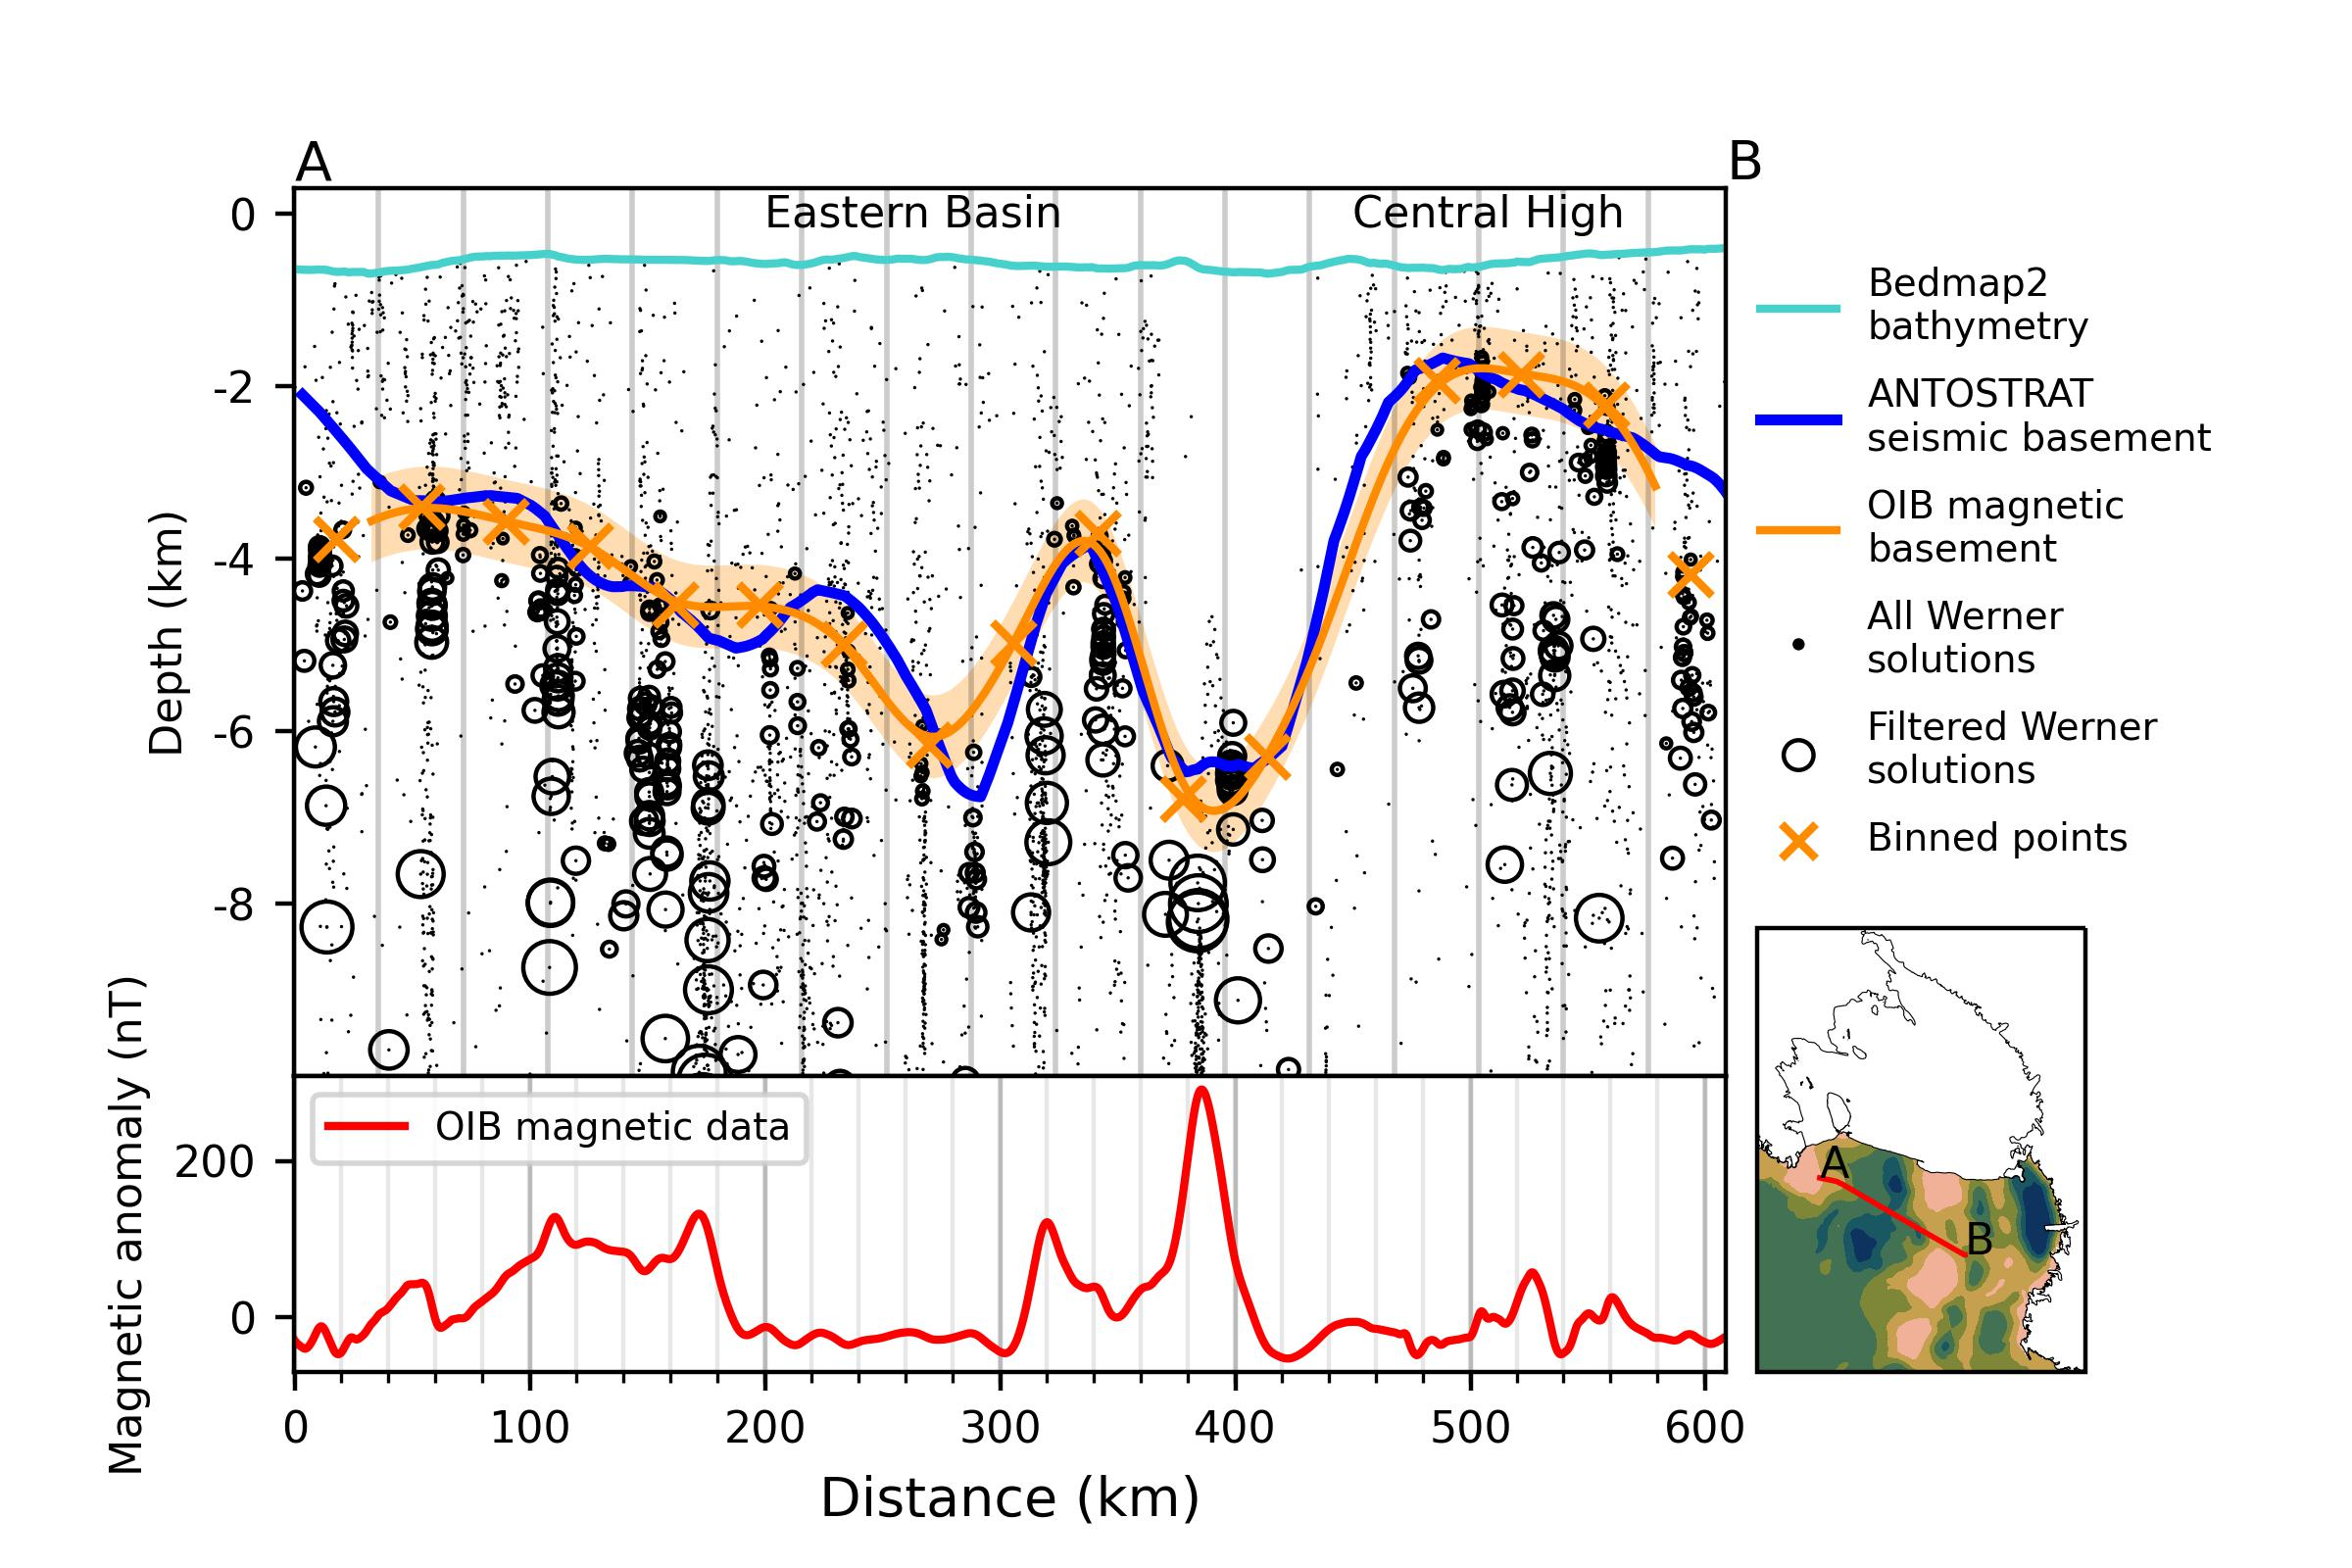
\includegraphics[width=\textwidth]{figures/chp2/Fig2_OIB_403_1.jpg}
    \caption[Ross Sea magnetic and seismic basement comparison]{Ross Sea magnetic and seismic basement comparison. Operation IceBridge airborne magnetic data (lower panel) from segment 403.1 used in Werner deconvolution to produce magnetic anomaly source solutions (black dots). Filtering removed shallow solutions, and remaining solutions (circles scaled to magnetic susceptibility) were binned and interpolated to produce the magnetic basement (orange line with uncertainty band).}
    \label{fig:chp2_OIB_403_1}
\end{figure}

Our RIS results (Figure \ref{fig:appA_S4}) were merged with offshore ANTOSTRAT data \citep{brancolinidescriptive1995} and smoothed with an 80~km Gaussian filter to match the characteristic wavelengths of the Ross Sea basement (Section \ref{appA:text_S5}). The combined grid (Figure \ref{fig:chp2_Basement_sediment}a) was then subtracted from BedMachine bathymetry \citep[Figure \ref{fig:chp2_Bathy_Mag}a, Section \ref{appA:text_S6},][]{morlighemdeep2020}, to obtain the sediment thickness distribution for the Ross Embayment (Figure \ref{fig:chp2_Basement_sediment}b).\\

These sub-RIS results together with free-air gravity data allowed us to infer the locations of regional scale faults beneath the RIS. Criteria used to locate faults include 1) high relief on the magnetic basement surface, 2) linear trends that cross zones of shallow basement, 3) high gradient gravity anomalies (Figure \ref{fig:appA_S1}a, ROSETTA-Ice) and 4) large contrasts in sediment thickness. Narrow, deep, linear basins are likely to be controlled by active faults \citep[e.g.][]{finnexamples2002, drenthshallow2019}. We display the inferred faults upon a base map of crustal stretching factors ($\beta$-factor; the ratio of crustal thickness before and after extension, Figure \ref{fig:chp2_Tectonic_interpretation}a), using an initial crustal thickness of 38~km \citep{müllereocene2007}, a continent-wide Moho model \citep{ansvelocity2015}, and our basement surface as the top of the crust (Section \ref{appA:text_S6}).


\section{Results}

We find that an almost continuous drape of sediment covers the RIS region (Figure \ref{fig:chp2_Basement_sediment}b), with only $\sim$3\% of the area having \textless 200~m of sedimentary cover. Prominent beneath the midline of the RIS is a broad NNW-SSE trending basement ridge (Figure \ref{fig:chp2_Basement_sediment}a, Mid-Shelf High; MSH), which comprises most of the shallowest (\textless 700 meters below sea level (mbsl)) sub-RIS basement, with several regions with as little as 100~m of sedimentary cover. Basement is deeper on the East Antarctic side of the MSH, where it averages $\sim$2400~mbsl, compared to an average depth of $\sim$1900~mbsl on the West Antarctic side (Figure \ref{fig:chp2_Basement_sediment}a histogram). Sedimentary fill is $\sim$400~m greater and more uniformly distributed on the East Antarctic side than the West Antarctic side (Figure \ref{fig:chp2_Basement_sediment}b histogram).\\

To estimate our uncertainty (Section \ref{appA:text_S7}), we examined the misfit between OIB and ANTOSTRAT basement (Figures \ref{fig:chp2_OIB_403_1} \& \ref{fig:appA_S2}) and between our basement and OIB basement (Figures \ref{fig:appA_S3}e\&f). There is a median misfit of 480~m (22\% of average RIS depth) for basement (Figures \ref{fig:appA_S5} \& \ref{fig:appA_S6}). A similar 470~m median basement misfit is estimated by comparing our results to eight active source seismic surveys (Figure \ref{fig:chp2_Basement_sediment}b, Table \ref{table:appA_S1}). Incorporating the $\sim$70~m uncertainty in the bathymetry model \citep{tintoross2019}, our representative sediment thickness uncertainty is 550~m (37\% of average RIS thickness, Figure \ref{fig:appA_S5}).

\begin{figure}
    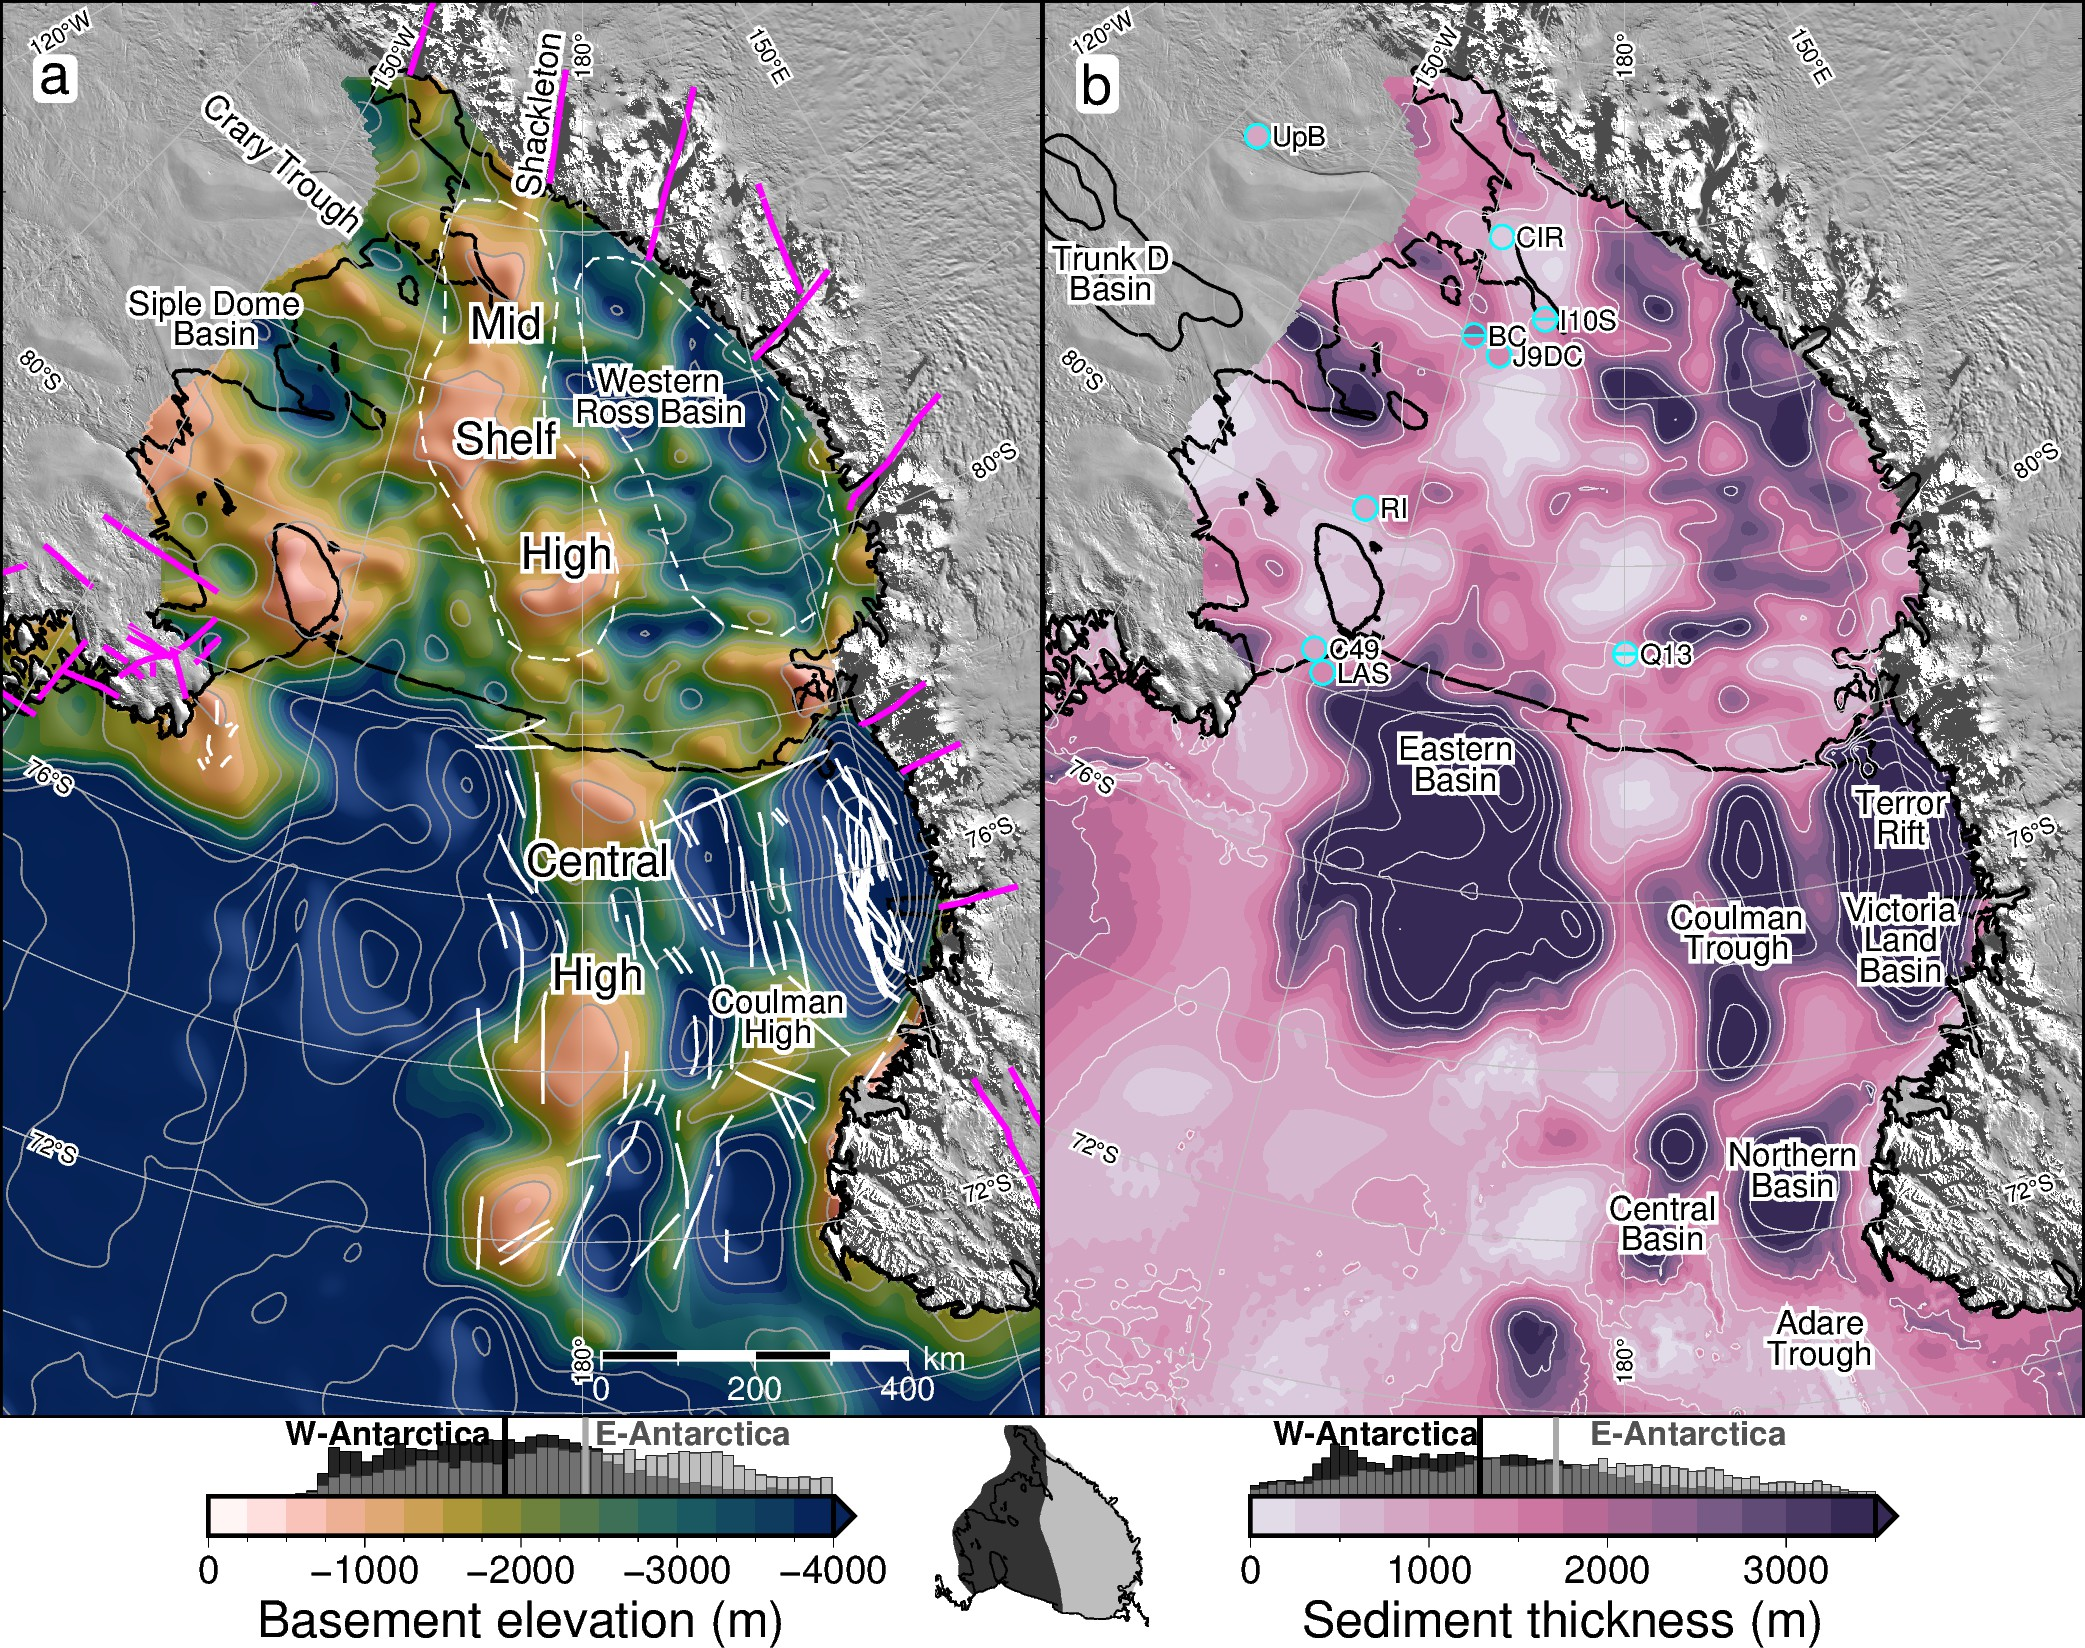
\includegraphics[width=\textwidth]{figures/chp2/Fig3_basement_sediment.jpg}
    \caption[Basement elevation and sediment thickness]{\textbf{(a)} Basement elevation (magnetic for Ross Ice Shelf (RIS), seismic elsewhere) contoured at 1~km intervals. Pink lines are onshore mapped and inferred faults \citep{goodgegeological2020, siddowaytectonics2008, ferraccioliaeromagnetic2002a}. White lines are offshore faults \citep{salvinicenozoic1997, luyendykstructural2001, chiappiniregional2002, saulineogene2021}. Dashed white lines show Mid Shelf High and Western Ross Basin extents. \textbf{(b)} Sediment thickness contoured at 1~km intervals. Previous basement-imaging RIS seismic surveys (cyan circles, Table \ref{table:appA_S1}) are plotted on same color scale, with upper and lower uncertainty ranges as circle halves, where reported. Trunk D Basin outlined in West Antarctica \citep{bellidentifying2006}. Color scales for both a) and b) are set to sub-RIS data range. Colorbar histograms show data distribution for East vs West Antarctic sides of the sub-RIS, separated by the Mid-Shelf High. Inset map shows East vs West divide. Vertical lines on histograms denote average values of each side.}
    \label{fig:chp2_Basement_sediment}
\end{figure}

A single broad and deep basin (300~x~600~km) separates the MSH and the Transantarctic Mountains (TAM) (Figure \ref{fig:chp2_Basement_sediment}a, Western Ross Basin). The Western Ross Basin parallels the TAM and has the deepest-observed sub-RIS basement depths of 4500~mbsl, accommodating sediments up to 3800~m thick (Figure \ref{fig:chp2_Basement_sediment}b). It contains a long, narrow NW-SE trending ridge with $\sim$1500~m structural relief above the basement sub-basins on either side. Bordering the MSH on the east, an elongate NW-SE trending basin runs from the RIS calving front to the Siple Coast GZ (Figure \ref{fig:chp2_Basement_sediment}a), where beneath Siple Dome we discover a 100~x~200~km depocenter reaching basement depths up to 4000~mbsl, with sediments up to 3700~m thick. We refer to this depocenter as Siple Dome Basin, a feature bounded on the east by a basement high that trends southward from Roosevelt Island. This high rises to its shallowest point at the GZ, where its sedimentary cover is less than 100~m. A second deep, narrow basin (50~x~200~km in dimension) is found along the north margin of Crary Ice Rise, separated from the Siple Dome Basin by an NW-SE ridge underlying Kamb Ice Stream. The basin, labelled Crary Trough in Figure \ref{fig:chp2_Basement_sediment}a, reaches basement depths of 3200~mbsl, with sediments 1800-2700~m thick. The southernmost RIS has an additional depocenter with up to 2000~m of fill beneath Whillans Ice Stream (location in Figure \ref{fig:chp2_Bathy_Mag}a).\\

Inferred active sub-RIS faults (Figures \ref{fig:chp2_Tectonic_interpretation}a \& \ref{fig:appA_S1}) correspond to narrow, linear basement basins with high-gradient gravity anomalies, prevalent on the West Antarctic side (Figure \ref{fig:appA_S1}a). Inactive normal and strike-slip faults are inferred along lineaments that segment the shallow MSH into blocks and are oriented parallel to TAM outlet glacier faults. $\beta$-factors are indicative of thinned crust and are different on either side of the MSH. The TAM side shows higher $\beta$-factors (average 1.99) with low variability. The West Antarctic side has lower $\beta$-factors overall (average 1.82), but with some higher values up to 2.1 (Figure \ref{fig:chp2_Tectonic_interpretation}a). 



\section{Discussion}

Sub-RIS sedimentary basins align with and show lateral continuity with the Ross Sea’s Roosevelt Sub-Basin, Eastern Basin, Coulman Trough, and Victoria Land Basin \citep[Figure \ref{fig:chp2_Basement_sediment}, e.g.][]{coopergeology1995}. The MSH passes northward into the Ross Sea's prominent Central High (CH). At the southern RIS margin, the narrow Siple Dome Basin has continuity with the previously identified Trunk D Basin \citep[Figure \ref{fig:chp2_Basement_sediment}a,][]{bellidentifying2006}. The throughgoing trends imply regional continuity of crustal structure and a common tectonic development of the Ross Sea and RIS regions. Our sediment thicknesses are compatible with those determined by a) eight active-source seismic surveys (Figure \ref{fig:chp2_Basement_sediment}b), for which the median misfit is 470~m (Table \ref{table:appA_S1}), and b) surface wave dispersion indicating 2-4~km of sediment under the RIS, similar to our range, with the maximum beneath Crary Ice Rise \citep{zhouradial2022}. Three additional western RIS seismic profiles report up to several kilometers of sediment, in general accordance with our results \citep{sternlithospheric1991, tenbrinkgeophysical1993, beaudoincharacteristics1992}. Additionally, machine learning applied to geophysical datasets predicts a high likelihood of sedimentary basins at the locations of Siple Dome Basin and Crary Trough \citep{lisedimentary2022}.

\subsection{West Antarctic Rift System extensional basins}
The Western Ross Basin has a configuration similar to the western Ross Sea rift basins \citep[e.g.][]{salvinicenozoic1997} with a broad and deep basin, separated into distinct depocenters by a linear, low relief ridge. The deeper of the depocenters, on the TAM side of the ridge, coincides with alternating high and low free-air gravity anomalies (Figure \ref{fig:appA_S1}a). These similarities suggest the sub-RIS continuations of  Coulman Trough and Victoria Land Basin (Figure \ref{fig:chp2_Basement_sediment}b) likely share a common tectonic origin as fault-controlled basins (Figures \ref{fig:chp2_Basement_sediment}a \& \ref{fig:chp2_Tectonic_interpretation}a) formed through Cretaceous distributed continental extension across the WARS \citep{jordangeological2020}. These sub-RIS basins terminate against the southern segment of the MSH (Figure \ref{fig:chp2_Basement_sediment}a).\\

The linear ridge within the Western Ross Basin (Figure \ref{fig:chp2_Basement_sediment}a) may be an expression of normal or oblique faults linked to the southward-narrowing Terror Rift \citep{saulineogene2021}, formed due to Cenozoic oceanic spreading in the Adare Trough \citep[Figure \ref{fig:chp2_Basement_sediment}b,][]{granotlate2018}. The Western Ross Basin, with up to 3800~m of fill, terminates along the prominent edge of the MSH that lines up with the fault-controlled trough and crustal boundary that passes southward beneath Shackleton Glacier \citep{borgisotopic1990}. We interpret the basement lineament (Figure \ref{fig:chp2_Tectonic_interpretation}a) as a transfer fault separating sectors of crust extended to different degrees. \\

\begin{figure}
    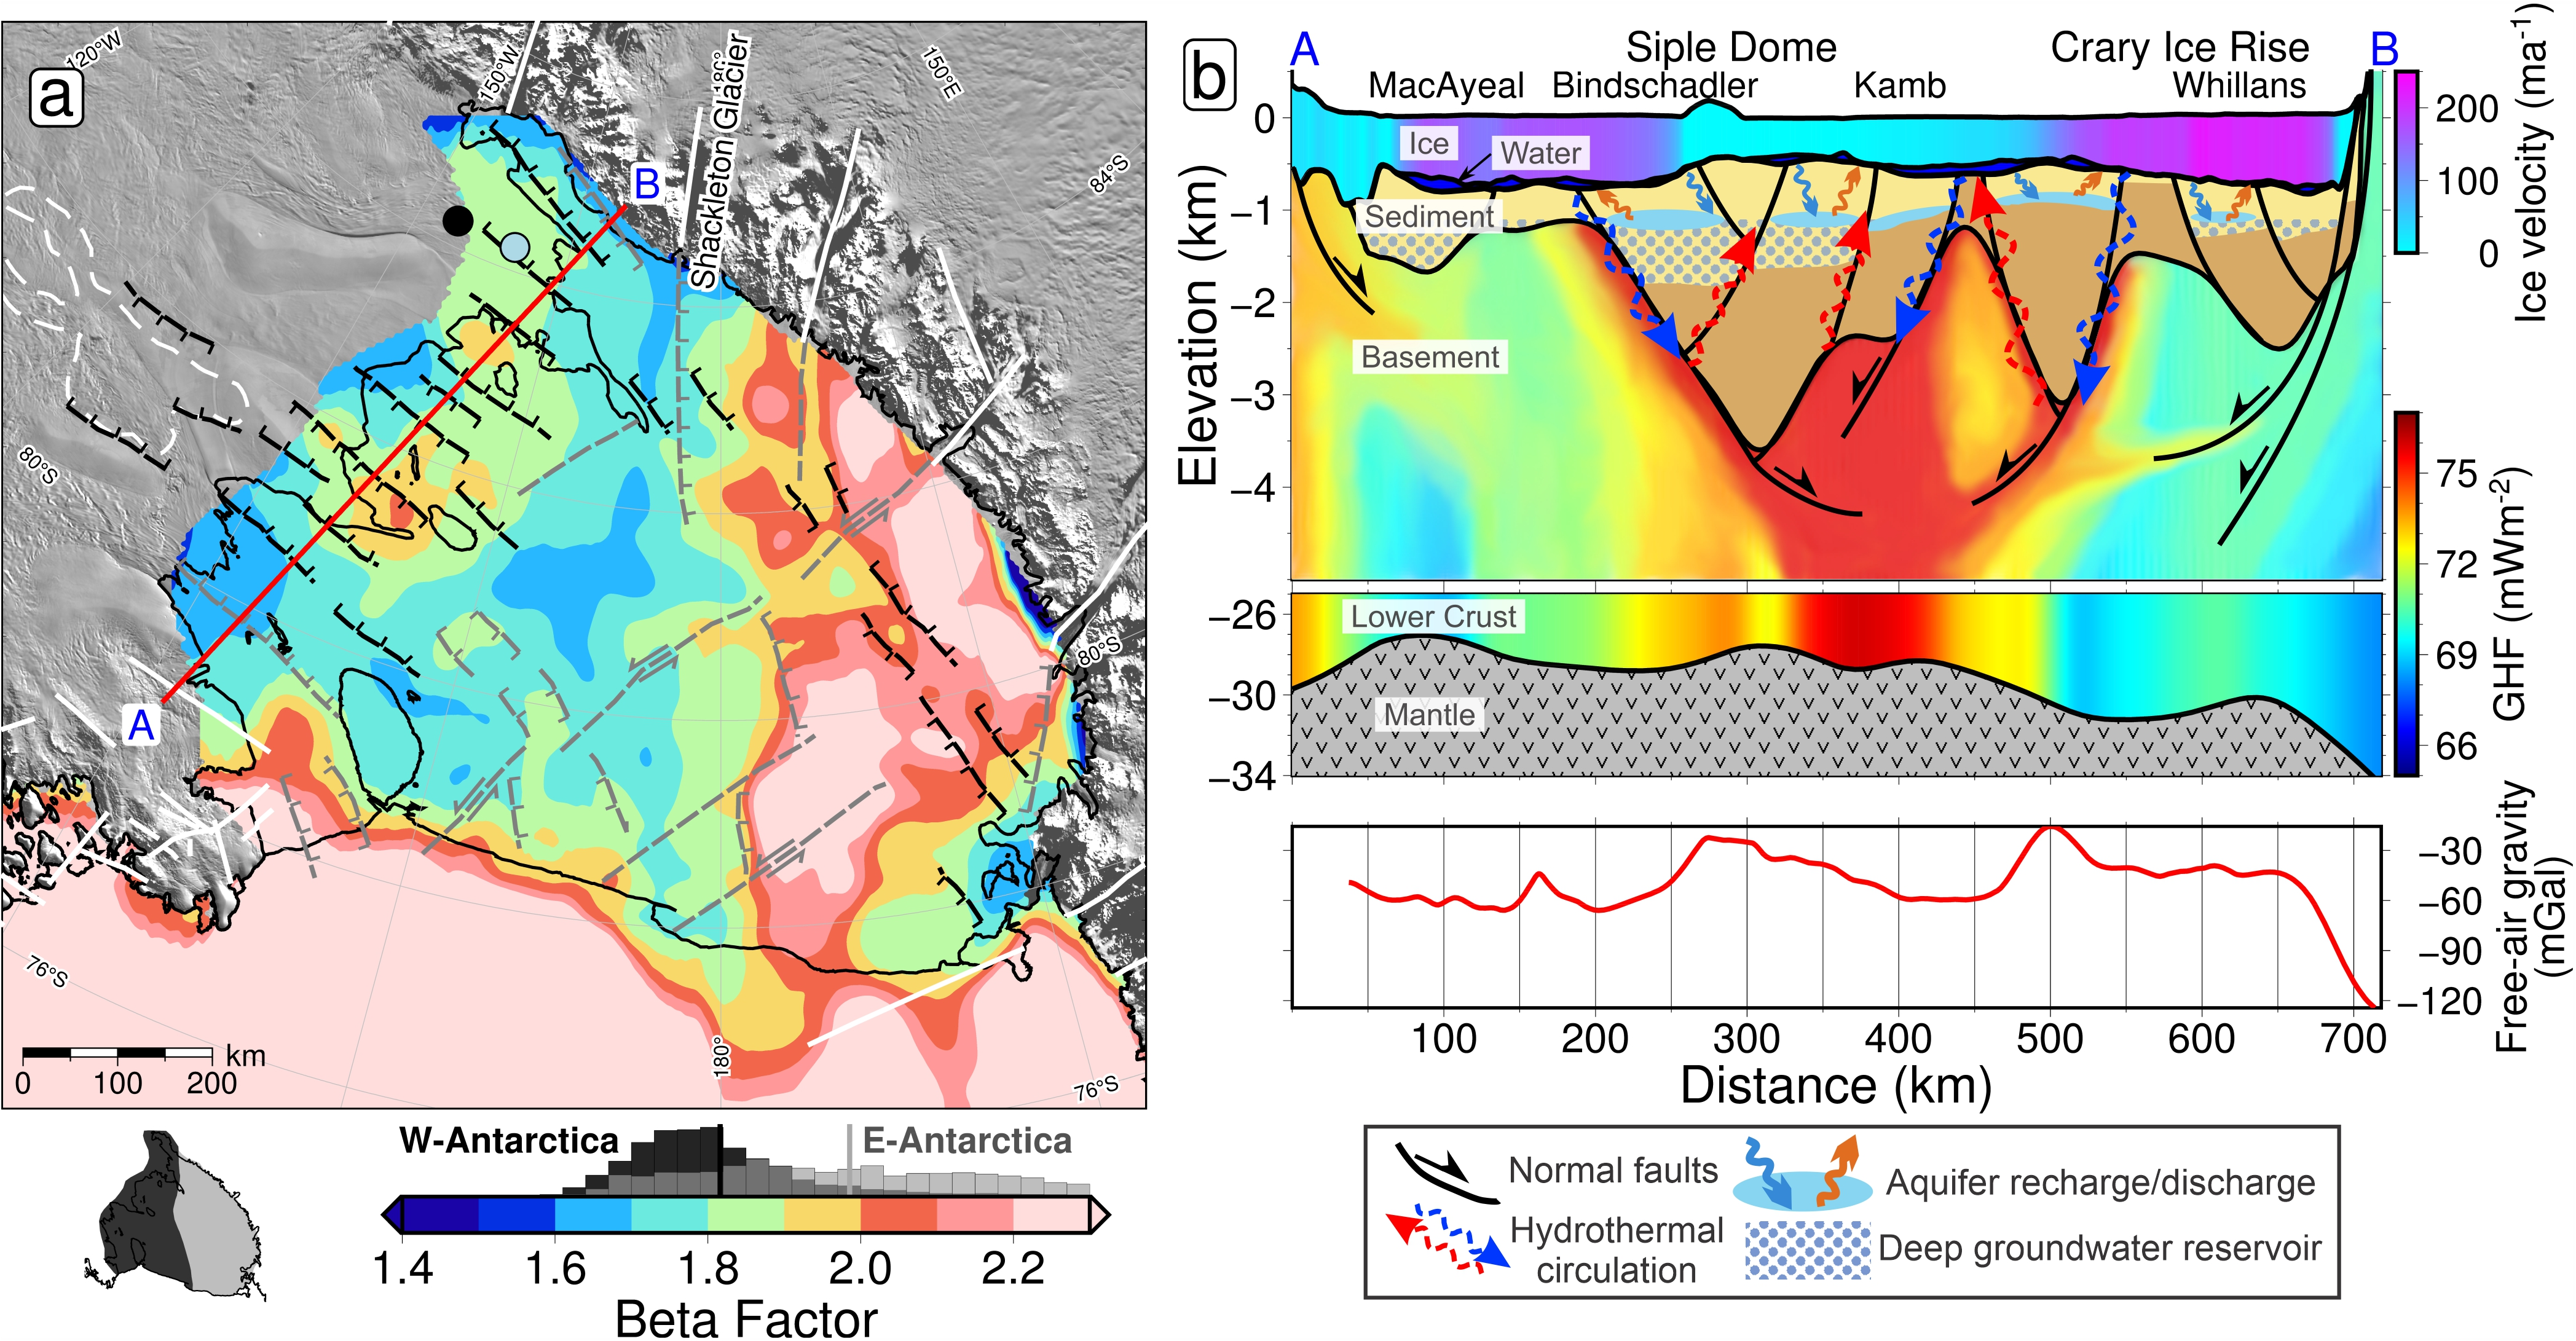
\includegraphics[width=\textwidth]{figures/chp2/Fig4_tectonic_interpretation.jpg}
    \caption[Tectonic interpretation of the sub-Ross Ice Shelf]{Tectonic interpretation of the sub-Ross Ice Shelf (RIS). 
    \textbf{(a)} $\beta$ stretching factors (Section \ref{appA:text_S6}). Colorbar histogram shows data distribution of West vs. East Antarctic sides, same as Figure \ref{fig:chp2_Basement_sediment}. Black and grey lines indicate inferred active and inactive faults, respectively, with kinematics shown with half-arrows (strike or oblique-slip) and hachures (normal-sense). White lines show previously reported faults, same as Figure \ref{fig:chp2_Basement_sediment}a. Dashed-white outline is Trunk D Basin \citep{bellidentifying2006}. Black and blue dots show Subglacial Lake Whillans and sedimentary basin from \citet{gustafsondynamic2022}, respectively. Cross-section A-B in red. \textbf{(b)} Siple Coast cross-section from A-B, showing basin sediments bounded by faults, with geothermal heat flux (GHF) through the crust (lower panel from \citet{burton-johnsongeothermal2020}, upper panel interpreted). Ice surface, ice base, and bathymetry from \citet{morlighemdeep2020}. Ice streams coloured by velocity \citep{mouginotcontinent2019, venturellimid2020}. Moho is from \citet{shencrust2018}. Lower panel shows ROSETTA-Ice gravity. Named features are labelled on top.} 
    \label{fig:chp2_Tectonic_interpretation}
\end{figure}

The southeastern RIS margin is distinguished by linear ridges and narrow, deep basins. The prominent NW-SE basement trends coincide with high-gradient gravity anomalies \citep[Figure \ref{fig:appA_S1}a,][]{tintoross2019} and thick sediments, suggesting normal fault control and active divergent tectonics beneath the GZ. Our Siple Coast cross-section (Figure \ref{fig:chp2_Tectonic_interpretation}b) displays dramatic basement relief, exceeding 2~km, in the Siple Dome Basin and Crary Trough, which we attribute to displacement upon high angle faults. Portions of basin-bounding faults were previously detected by ground-based gravity surveys upon the Whillans Ice Stream flank \citep[Figure \ref{fig:chp2_Tectonic_interpretation}a,][]{mutobathymetry2013} and site J9DC (Figure \ref{fig:chp2_Basement_sediment}b), where large variations in sediment thickness indicate up to 600~m of fault throw \citep{greischaranalysis1992}. The continuity between the narrow Siple Dome Basin (this study) and the Trunk D Basin \citep[Figure \ref{fig:chp2_Basement_sediment}a,][]{bellidentifying2006} suggests that the active tectonic domain continues southward past the GZ. The fault-controlled tectonic basins may reflect a crustal response to the lithospheric foundering hypothesized beneath the South Pole region \citep{shenseismic2018} or be a broader regional expression of Neogene extension that formed the Bentley Subglacial Trench \citep{lloydseismic2015}.

\subsection{Consequences for ice sheet dynamics}

Our basement topography and suggested crustal faults likely exert a strong influence on the overriding ice, especially along the Siple Coast. Here, we show deep and thick sedimentary basins which likely contain voluminous basinal aquifers \citep[Figure \ref{fig:chp2_Tectonic_interpretation}b; cf.][]{gustafsondynamic2022}. Where these aquifers discharge along fault-damage zones, they can enhance GHF and promote basal melting \citep{goochpotential2016}, as depicted in Figure \ref{fig:chp2_Tectonic_interpretation}a. The elevated GHF seen at Subglacial Lake Whillans \citep[285~mW/m\textsuperscript{2},][]{fisherhigh2015} may arise from fault localization (Figure \ref{fig:chp2_Tectonic_interpretation}a). Confinement of the aquifers between the ice bed and low-permeability basement may promote fluid overpressure, enabling ice streaming \citep[e.g.][]{ravierglaciohydrogeology2018}. Additionally, the Siple Coast faults likely accommodate the solid Earth's response to fluctuating ice volume. A matter receiving considerable debate \citep{neuhausdid2021, venturellimid2020, lowrydeglacial2019}, is Kingslake et al.'s \citeyear{kingslakeextensive2018} finding of rapid re-advance of the Siple Coast GZ following Holocene deglaciation. The re-advance was in part due to swift glacioisostatic rebound \citep[cf.][]{lowrygeologic2020, couloncontrasting2021}, a process aided by the region’s low-viscosity mantle \citep{whitehousesolid2019} and likely to be accommodated upon pre-existing crustal faults, as observed in the Lambert Graben \citep{phillipsbrittle2009}. Our proposed graben-bounding faults would provide a tectonic control on the glacioisostatic adjustment of the Siple Coast region.

\subsection{Mid-Shelf High - Central High}
The 650-km-long Mid-Shelf High features three shallow, blocky segments \textgreater150~km in breadth, which have only thin sediment cover (\textless200~m). At their shallowest points, the top of basement  lies within $\sim$300~m  of the ice shelf base, at a depth comparable to the basement high at Roosevelt Island. Roosevelt Island is a modern pinning point \citep{stillmechanical2019} owing to the thicker sediment, there (Figure \ref{fig:chp2_Basement_sediment}b). We introduce the MSH as a prominent pinning point at times of advance and greater extent of the Antarctic Ice Sheet, in keeping with evidence from subglacial sediment records that indicate a major ice flow divide between East and West Antarctic ice during and since Last Glacial Maximum \citep{liapatite2020, lichtupb2014, coenenpaleogene2019}. \\

The prominence of the MSH is due in part to the contrasting geologic properties of the East versus West Antarctic type crust and their respective responses to WARS extension. We distinguished $\beta$-factors on the TAM-side that are high and uniform, indicating distributed crustal extension. The West Antarctic side displays lower $\beta$-factors overall, but with localized extreme thinning beneath Siple Coast (Figure \ref{fig:chp2_Tectonic_interpretation}a). The greater amount of extension on the East Antarctic side coincides with the deeper bathymetry (Figure \ref{fig:chp2_Bathy_Mag}a), deeper basement, and thicker sediments (Figure \ref{fig:chp2_Basement_sediment}). The contrasting properties are also evident in ROSETTA-Ice magnetic and gravity anomalies, used by \citet{tintoross2019} to identify a north-south trending tectonic boundary along the midline of Ross Embayment. The MSH in the magnetic basement coincides with and spans this boundary, which has been further substantiated by passive-seismic studies that show a lithospheric-scale boundary \citep{chenganisotropy2021, white-gaynorheterogeneous2019}. To the north, the features continue into the Ross Sea’s Central High. Southward, the MSH basement feature trends into the TAM, where its western edge aligns with Shackleton Glacier, occupying a major fault separating the distinct geologic domains of the central and southern TAM \citep{borgisotopic1990, paulsenstructure2004}, which also parallels a prominent magnetic lineament at the South Pole \citep{studingercrustal2006}. The structure may be an expression of the East Antarctic craton margin or a major intracontinental transform \citep[Figure \ref{fig:chp2_Tectonic_interpretation}a,][]{studingercrustal2006}. \\

At the time of Oligocene initiation of the Antarctic Ice sheet, paleotopographic reconstructions of the proto-Ross Embayment depict a long, broad range, emergent above sea level \citep{paxmanreconstructions2019, wilsonantarctic2012}, that we equate to the MSH-CH that divides the Embayment. The CH hosted small ice caps with alpine glaciers formed during the initial glacial stage in the region \citep{desantisseismic1995}, and continental ice expanded to the outer Ross Sea continental shelf from those centres \citep{bartglacial2012}. Between the late Oligocene and mid-Miocene, the CH subsided by up to 500~m \citep{leckielate1983, kulhanekrevised2019}, receiving 100’s of meters of sediment cover \citep[$\sim$400~m at DSDP 270;][]{desantisseismic1995}. The geophysical similarities and continuity between the Ross Sea’s CH and the RIS’s MSH imply a similar glaciation and subsidence history for the MSH. A terrestrial/alpine stage for the MSH helps to explain the region’s potential to hold the late Oligocene’s larger-than-modern ice volumes \citep{wilsoninitiation2013, pekarresolving2006}, with the MSH-CH having a central role in Oligocene ice sheet development and the subsequent evolution of the ice sheet and ice shelf, as is documented in the Ross Sea \citep{halberstadticesheet2016}.

\subsection{Thermal subsidence and sedimentation}
Incorporating the updated basement basin extents and geometries into post-rift thermal subsidence modelling will enable better-constrained paleotopographic reconstructions. For the sub-RIS, these reconstructions \citep{wilsonantarctic2012, paxmanreconstructions2019} use a post-Eocene subsidence model based on gravity-derived basin geometries and uniform $\beta$-factors \citep{wilsonwest2009}. This model predicts uniform stretching of the eastern sub-RIS from the ice front to the Siple Coast, while our $\beta$-factors show increasing stretching from the ice front to the Siple Coast. This observed additional thinning likely has resulted in more subsidence for Siple Dome and the north flank of Crary Ice Rise, which can now be accounted for in reconstructions. Our sediment thickness comparison with past models \citep[Section \ref{appA:text_S6},][]{wilsonwest2009} shows the majority of the sub-RIS, especially the Siple Coast, contains more total sediment than previously estimated (Figure \ref{fig:appA_S1}f). Depending on the age of this sediment, reconstructions may need to account for the additional sediment deposition and loading.

\section{Conclusions}
Here we present a depth to magnetic basement map for the Ross Ice Shelf (RIS) from Werner deconvolution of airborne magnetic data. The RIS magnetic basement is tied to Ross Sea seismic basement, providing the first synthetic view of Ross Embayment crustal structure. Using a bathymetry model, we obtain the sediment thickness distribution and calculate crustal extension factors for the sub-RIS. The extensional features we image, resulting from West Antarctic Rift System extension, have continuity with Ross Sea basement structures to the north, and the prominent Mid-Shelf High trends northward into the Ross Sea’s Central High. This combined high separates East and West Antarctic type crust, affected by different degrees of continental extension. The Mid-Shelf High was likely subaerial in the Oligocene, able to support alpine ice caps in early Antarctic glaciation. Subsequently, it formed a prominent pinning point and ice flow divide between the East and West Antarctic Ice Sheets. \\

Newly identified narrow, linear, deep sedimentary basins provide evidence of active faults beneath the Siple Coast grounding zone, where thinned crust overlying anomalous mantle \citep{shencrust2018} likely experiences elevated geothermal heat flow promoting the formation of subglacial water. Faults that control basement margins may accommodate motion caused by the glacioisostatic response to ice sheet volume changes. Subglacial sedimentary basins in this setting likely contain confined aquifers within permeable basin fill. Here, ice overburden pressure would control flow both between and within the subglacial and groundwater systems, possibly localizing geothermal heat. Updated sediment thickness and basin extents should be incorporated into new paleotopographic reconstructions of time intervals of interest for paleo-ice sheet modelling. Our work contributes critical information about Ross Embayment basement topography and subglacial boundary conditions that arise from an interplay of geology, tectonics, and glaciation.


\section{Open Research}
ROSETTA-Ice and Operation IceBridge magnetics data are available through \url{https://www.usap-dc.org/view/project/p0010035} and \url{https://nsidc.org/data/IMCS31b}, respectively. Results from this study are available to download from \url{https://doi.pangaea.de/10.1594/PANGAEA.941238} and a Jupyter notebook documenting our workflow and figure creation is available at \url{https://zenodo.org/badge/latestdoi/470814953}.

\section{Acknowledgements}

Funding support from the New Zealand Ministry of Business and Innovation and Employment through the Antarctic Science Platform contract (ANTA1801) Antarctic Ice Dynamics Project (ASP-021-01) and the National Science Foundation (1443497 and 1443534), and Antarctica New Zealand. We are grateful to Robin Bell, Isabel Cordero, Alec Lockett, Joel Wilner, Zoe Krauss, and the entire ROSETTA-Ice team for undertaking the ambitious data acquisition and processing effort. We thank Katharina Hochmuth and Guy Paxman for thoughtful reviews which greatly improved the manuscript, as well as Chris Sorlien, Tim Stern, Simon Lamb, Lara Pérez, Ryan Venturelli, Wei Ji Leong, and Dan Lowry for valuable input. Figures used GMT6/PyGMT \citep{wesselgeneric2019, uiedapygmt2021}, with a script adapted from \citet{venturellimid2020}. Geosoft Oasis Montaj\textsuperscript{TM} was used for magnetics processing and Werner deconvolution. Open access publishing facilitated by Victoria University of Wellington, as part of the Wiley - Victoria University of Wellington agreement via the Council of Australian University Librarians. \\

Chapter \ref{ch:2}, in full, is a reprint of material as it appears in Geophysical Research Letters: 
Tankersley, M. D., Horgan, H. J., Siddoway, C. S., Caratori Tontini, F., \& Tinto, K. J. (2022). Basement topography and sediment thickness beneath Antarctica's Ross Ice Shelf. \textit{ Geophysical Research Letters}, 49, e2021GL097371. \url{https://doi.org/10.1029/2021GL097371}. The only changes made from the published version include formatting and replacing preprint citations with accepted paper citations. I conceived the study with my co-authors, undertook the study and analysis, and wrote the manuscript myself.